\documentclass[review]{elsarticle}
%\usepackage[hidelinks]{hyperref}
\usepackage[hidelinks]{hyperref}
\usepackage[linesnumbered,ruled,vlined]{algorithm2e}
\usepackage[normalem]{ulem}
% \modulolinenumbers[5]
\usepackage[margin=1in]{geometry}
\usepackage{optidef}
\usepackage{adjustbox}


% \journal{EJOR}
\journal{Expert Systems with Applications}

\usepackage{tikz}
\usetikzlibrary{shapes.geometric, arrows}

\usepackage{amsmath,amsthm,amsopn,amstext,amscd,amsfonts,amssymb,lscape}
% \usepackage{color}
\usepackage{xcolor}
\usepackage{comment}
\usepackage{booktabs}
\usepackage{longtable}
%\usepackage{showframe}
%\usepackage{theorem}
\newtheorem{theorem}{\bf Theorem}[section]
\newtheorem{coro}{\bf Corollary}[section]

%%%%%%%%%%%%%%%%%%%%%%%
%% Elsevier bibliography styles
%%%%%%%%%%%%%%%%%%%%%%%
%% To change the style, put a % in front of the second line of the current style and
%% remove the % from the second line of the style you would like to use.
%%%%%%%%%%%%%%%%%%%%%%%

\tikzstyle{startstop} = [rectangle, rounded corners, 
minimum width=1cm, 
minimum height=1cm,
text centered, 
draw=black, 
fill=red!30]

\tikzstyle{io} = [trapezium, 
trapezium stretches=true, % A later addition
trapezium left angle=70, 
trapezium right angle=110, 
minimum width=3cm, 
minimum height=1cm, text centered, 
draw=black, fill=blue!30]

\tikzstyle{process} = [rectangle, 
minimum width=3cm, 
minimum height=1cm, 
text centered, 
text width=4cm, 
draw=black, 
fill=orange!30]

\tikzstyle{decision} = [diamond, 
minimum width=3cm, 
minimum height=1cm, 
text centered,
text width=4cm,
aspect=2,
draw=black, 
fill=green!30]
\tikzstyle{arrow} = [thick,->,>=stealth,  rounded corners]

%% Numbered
%\bibliographystyle{model1-num-names}

%% Numbered without titles
%\bibliographystyle{model1a-num-names}

%% Harvard
%\bibliographystyle{model2-names.bst}\biboptions{authoryear}

%% Vancouver numbered
%\usepackage{numcompress}\bibliographystyle{model3-num-names}

%% Vancouver name/year
%\usepackage{numcompress}\bibliographystyle{model4-names}\biboptions{authoryear}

%% APA style
\bibliographystyle{model5-names}\biboptions{authoryear}

%% AMA style
%\usepackage{numcompress}\bibliographystyle{model6-num-names}

%% `Elsevier LaTeX' style
% \bibliographystyle{elsarticle-num}
%%%%%%%%%%%%%%%%%%%%%%%
\definecolor{armygreen}{rgb}{0.19, 0.53, 0.43}
\newcommand{\JP}[1]{{\color{armygreen}#1}}
\newcommand{\CV}[1]{{\color{red}#1}}
\newcommand{\LA}[1]{{\color{blue}#1}}
\newcommand{\TP}[1]{{\color{orange}#1}}
\begin{document}

\begin{center}
	\begin{adjustbox}{width=1\textwidth,height=1\textheight,keepaspectratio}
	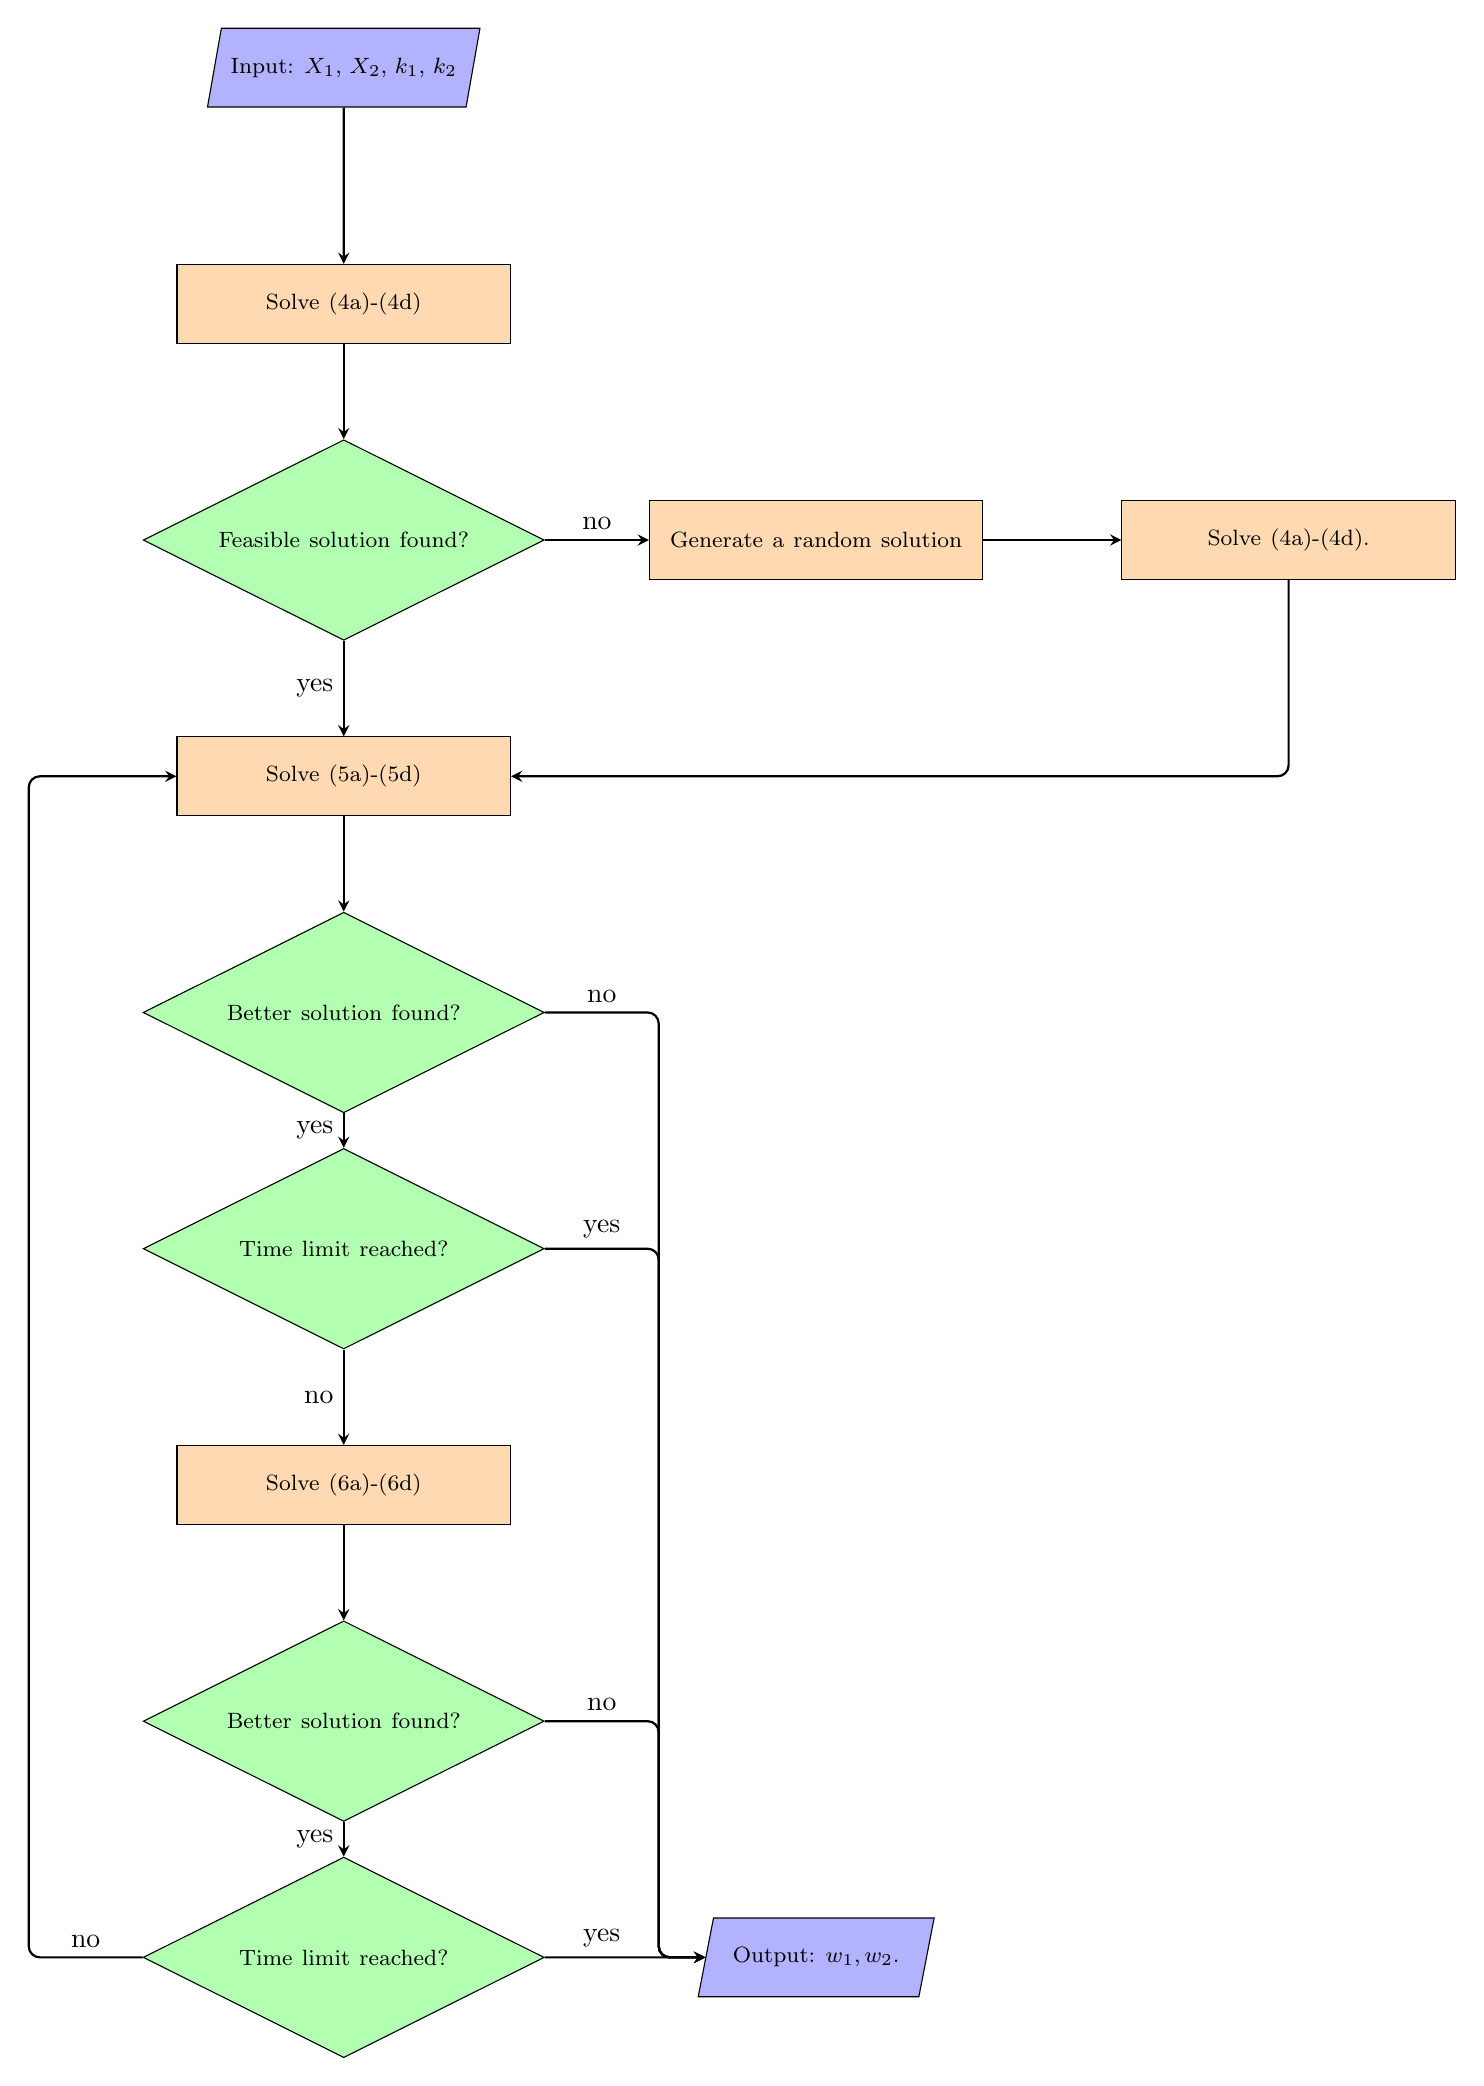
\begin{tikzpicture}[node distance=3cm, scale=1]
		
%	\node (start) [startstop] {\footnotesize Start};
	\node (in1) [io] {\footnotesize Input: $X_1$, $X_2$, $k_1$, $k_2$};
	\node (pro1) [process, below of=in1] {\footnotesize Solve (4a)-(4d)};
	%Time limit: $\tau/10$.};
	\node (dec1) [decision, below of=pro1] {\footnotesize Feasible solution found?};
	
	\node (pro2b) [process, right of=dec1, xshift=3cm] {\footnotesize Generate a random solution};
	\node (pro2c) [process, right of=pro2b, xshift=3cm] {\footnotesize Solve (4a)-(4d).};
	
	\node (pro2) [process, below of=dec1] {\footnotesize Solve (5a)-(5d)};
	
	\node (dec2a) [decision, below of=pro2] {\footnotesize Better solution found?};
	\node (dec2b) [decision, below of=dec2a] {\footnotesize Time limit reached?};
	
%	\node (out2a) [io, right of=dec2a, xshift=3cm] {\footnotesize Output};
%	\node (out2b) [io, right of=dec2b, xshift=3cm] {\footnotesize Output};
	
	\node (pro3) [process, below of=dec2b] {\footnotesize Solve (6a)-(6d)};
	
	\node (dec3a) [decision, below of=pro3] {\footnotesize Better solution found?};
	\node (dec3b) [decision, below of=dec3a] {\footnotesize Time limit reached?};
	
%	\node (out3a) [io, right of=dec3a, xshift=3cm] {\footnotesize Output};
	\node (out3b) [io, right of=dec3b, xshift=3cm] {\footnotesize Output: $w_1, w_2$.};
	
%	\node (dec2) [decision, below of=pro2a, yshift=-1cm] {\footnotesize hola}
%	\node (out1) [io, below of=pro2a] {Output};
%	\node (stop) [startstop, below of=out1] {Stop};
	
	% \draw [arrow] (start) -- (in1);
	\draw [arrow] (in1) -- (pro1);
	\draw [arrow] (pro1) -- (dec1);
	\draw [arrow] (dec1) -- node[anchor=east] {yes} (pro2);
	\draw [arrow] (dec1) -- node[anchor=south] {no} (pro2b);
	\draw [arrow] (pro2b) -- (pro2c);
	\draw [arrow] (pro2c) |- (pro2);
	\draw [arrow] (pro2) -- (dec2a);
	\draw [arrow] (dec2a) -- node[anchor=south] {no} +(4,0) |- (out3b);
	\draw [arrow] (dec2a) -- node[anchor=east] {yes} (dec2b);
	\draw [arrow] (dec2b) -- node[anchor=south] {yes} +(4,0) |- (out3b);
	\draw [arrow] (dec2b) -- node[anchor=east] {no} (pro3);
	\draw [arrow] (pro3) -- (dec3a);
	\draw [arrow] (dec3a) -- node[anchor=south] {no} +(4,0) |- (out3b);
	\draw [arrow] (dec3a) -- node[anchor=east] {yes} (dec3b);
	\draw [arrow] (dec3b) -- node[anchor=south] {yes} +(4,0) -- (out3b);
	\draw [arrow] (dec3b) -- node[anchor=south] {no} + (-4,0)  |-  (pro2);
%	\draw [arrow] (pro2a) -- (out1);
%	\draw [arrow] (out1) -- (stop);
	
\end{tikzpicture}
\end{adjustbox}
\end{center}


\begin{center}
	\begin{adjustbox}{width=1\textwidth,height=1\textheight,keepaspectratio}
		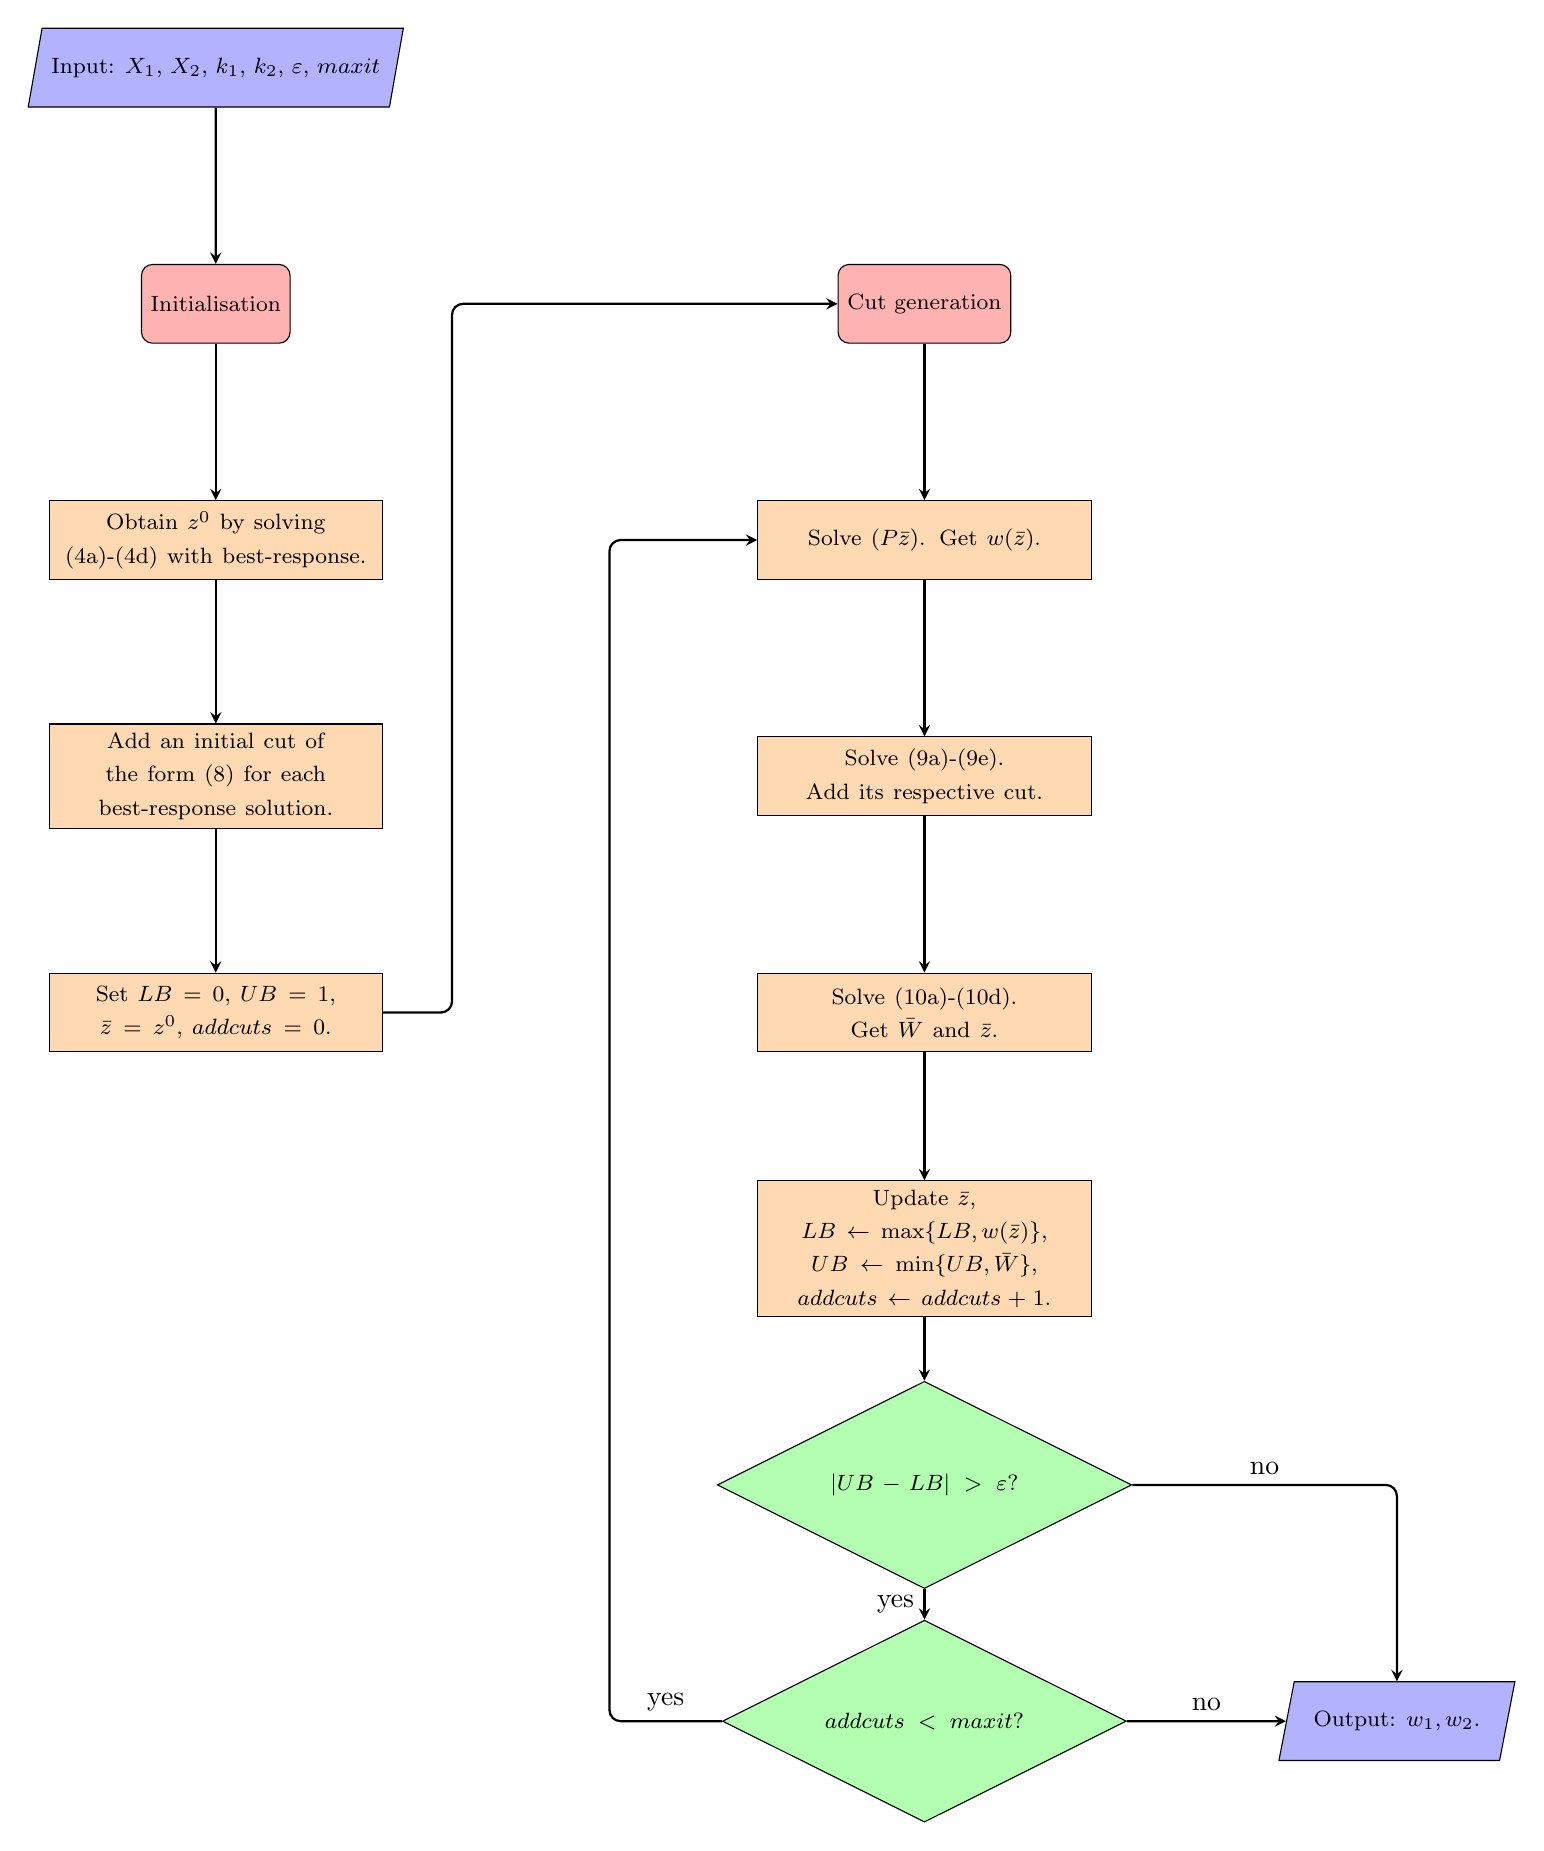
\begin{tikzpicture}[node distance=3cm, scale=1]
			
		%	\node (start) [startstop] {\footnotesize Start};
		\node (in1) [io] {\footnotesize Input: $X_1$, $X_2$, $k_1$, $k_2$, $\varepsilon$, $maxit$};
		
		\node (start) [startstop, below of=in1] {\footnotesize Initialisation};
		
		\node (pro1) [process, below of=start] {\footnotesize Obtain $z^0$ by solving (4a)-(4d) with best-response. };
		
		\node (pro2) [process, below of=pro1] {\footnotesize Add an initial cut of the form (8) for each best-response solution.};
		
		\node (pro3) [process, below of=pro2] {\footnotesize Set $LB=0$, $UB=1$, $\bar z = z^0$, $addcuts=0$.};
		
		\node (start2) [startstop, right of=start, xshift=6cm] {\footnotesize Cut generation};
		
		\node (pro4) [process, right of=pro1, xshift=6cm] {\footnotesize Solve $(P\bar z)$. Get $w(\bar z)$.};
		
		\node (pro5) [process, below of=pro4] {\footnotesize Solve (9a)-(9e). \\Add its respective cut.};
		
		\node (pro6) [process, below of=pro5] {\footnotesize Solve (10a)-(10d). Get $\bar W$ and $\bar z$.};
		
		\node (pro7) [process, below of=pro6] {\footnotesize Update $\bar z$, \\$LB\gets\max\{LB, w(\bar z)\}$, $UB\gets\min\{UB, \bar{W}\}$, $addcuts\gets addcuts+1$.};
		
		\node (dec7a) [decision, below of=pro7] {\footnotesize $|UB-LB| > \varepsilon$?};
		\node (dec7b) [decision, below of=dec7a] {\footnotesize $addcuts < maxit$?};
		
		\node (out) [io, right of=dec7b, xshift=3cm] {\footnotesize Output: $w_1, w_2$.};

		\draw [arrow] (in1) -- (start);
		\draw [arrow] (start) -- (pro1);
		\draw [arrow] (pro1) -- (pro2);
		\draw [arrow] (pro2) -- (pro3);
		\draw [arrow] (pro3) -- +(3,0) |- (start2) ;
		\draw [arrow] (start2) -- (pro4);
		\draw [arrow] (pro4) -- (pro5);
		\draw [arrow] (pro5) -- (pro6);
		\draw [arrow] (pro6) -- (pro7);
		\draw [arrow] (pro7) -- (dec7a);
		\draw [arrow] (dec7a) -- node[anchor=south] {no} +(6,0) -- (out);
		\draw [arrow] (dec7a) -- node[anchor=east] {yes} (dec7b);
		\draw [arrow] (dec7b) -- node[anchor=south] {no} (out);
		\draw [arrow] (dec7b) -- node[anchor=south] {yes} + (-4,0)  |-  (pro4);
		
%		\draw [arrow] (dec7b) -- node[]
		
%		\draw [arrow] (dec1) -- node[anchor=south] {no} (pro2b);
%		\draw [arrow] (pro2b) -- (pro2c);
%		\draw [arrow] (pro2c) |- (pro2);
%		\draw [arrow] (pro2) -- (dec2a);
%		\draw [arrow] (dec2a) -- node[anchor=south] {no} +(4,0) |- (out3b);
%		\draw [arrow] (dec2a) -- node[anchor=east] {yes} (dec2b);
%		\draw [arrow] (dec2b) -- node[anchor=south] {yes} +(4,0) |- (out3b);
%		\draw [arrow] (dec2b) -- node[anchor=east] {no} (pro3);
%		\draw [arrow] (pro3) -- (dec3a);
%		\draw [arrow] (dec3a) -- node[anchor=south] {no} +(4,0) |- (out3b);
%		\draw [arrow] (dec3a) -- node[anchor=east] {yes} (dec3b);
%		\draw [arrow] (dec3b) -- node[anchor=south] {yes} +(4,0) -- (out3b);
%		\draw [arrow] (dec3b) -- node[anchor=south] {no} + (-4,0)  |-  (pro2);
		%	\draw [arrow] (pro2a) -- (out1);
		%	\draw [arrow] (out1) -- (stop);
		
	\end{tikzpicture}
\end{adjustbox}
\end{center}

\begin{center}
	\begin{adjustbox}{width=1\textwidth,height=1\textheight,keepaspectratio}
		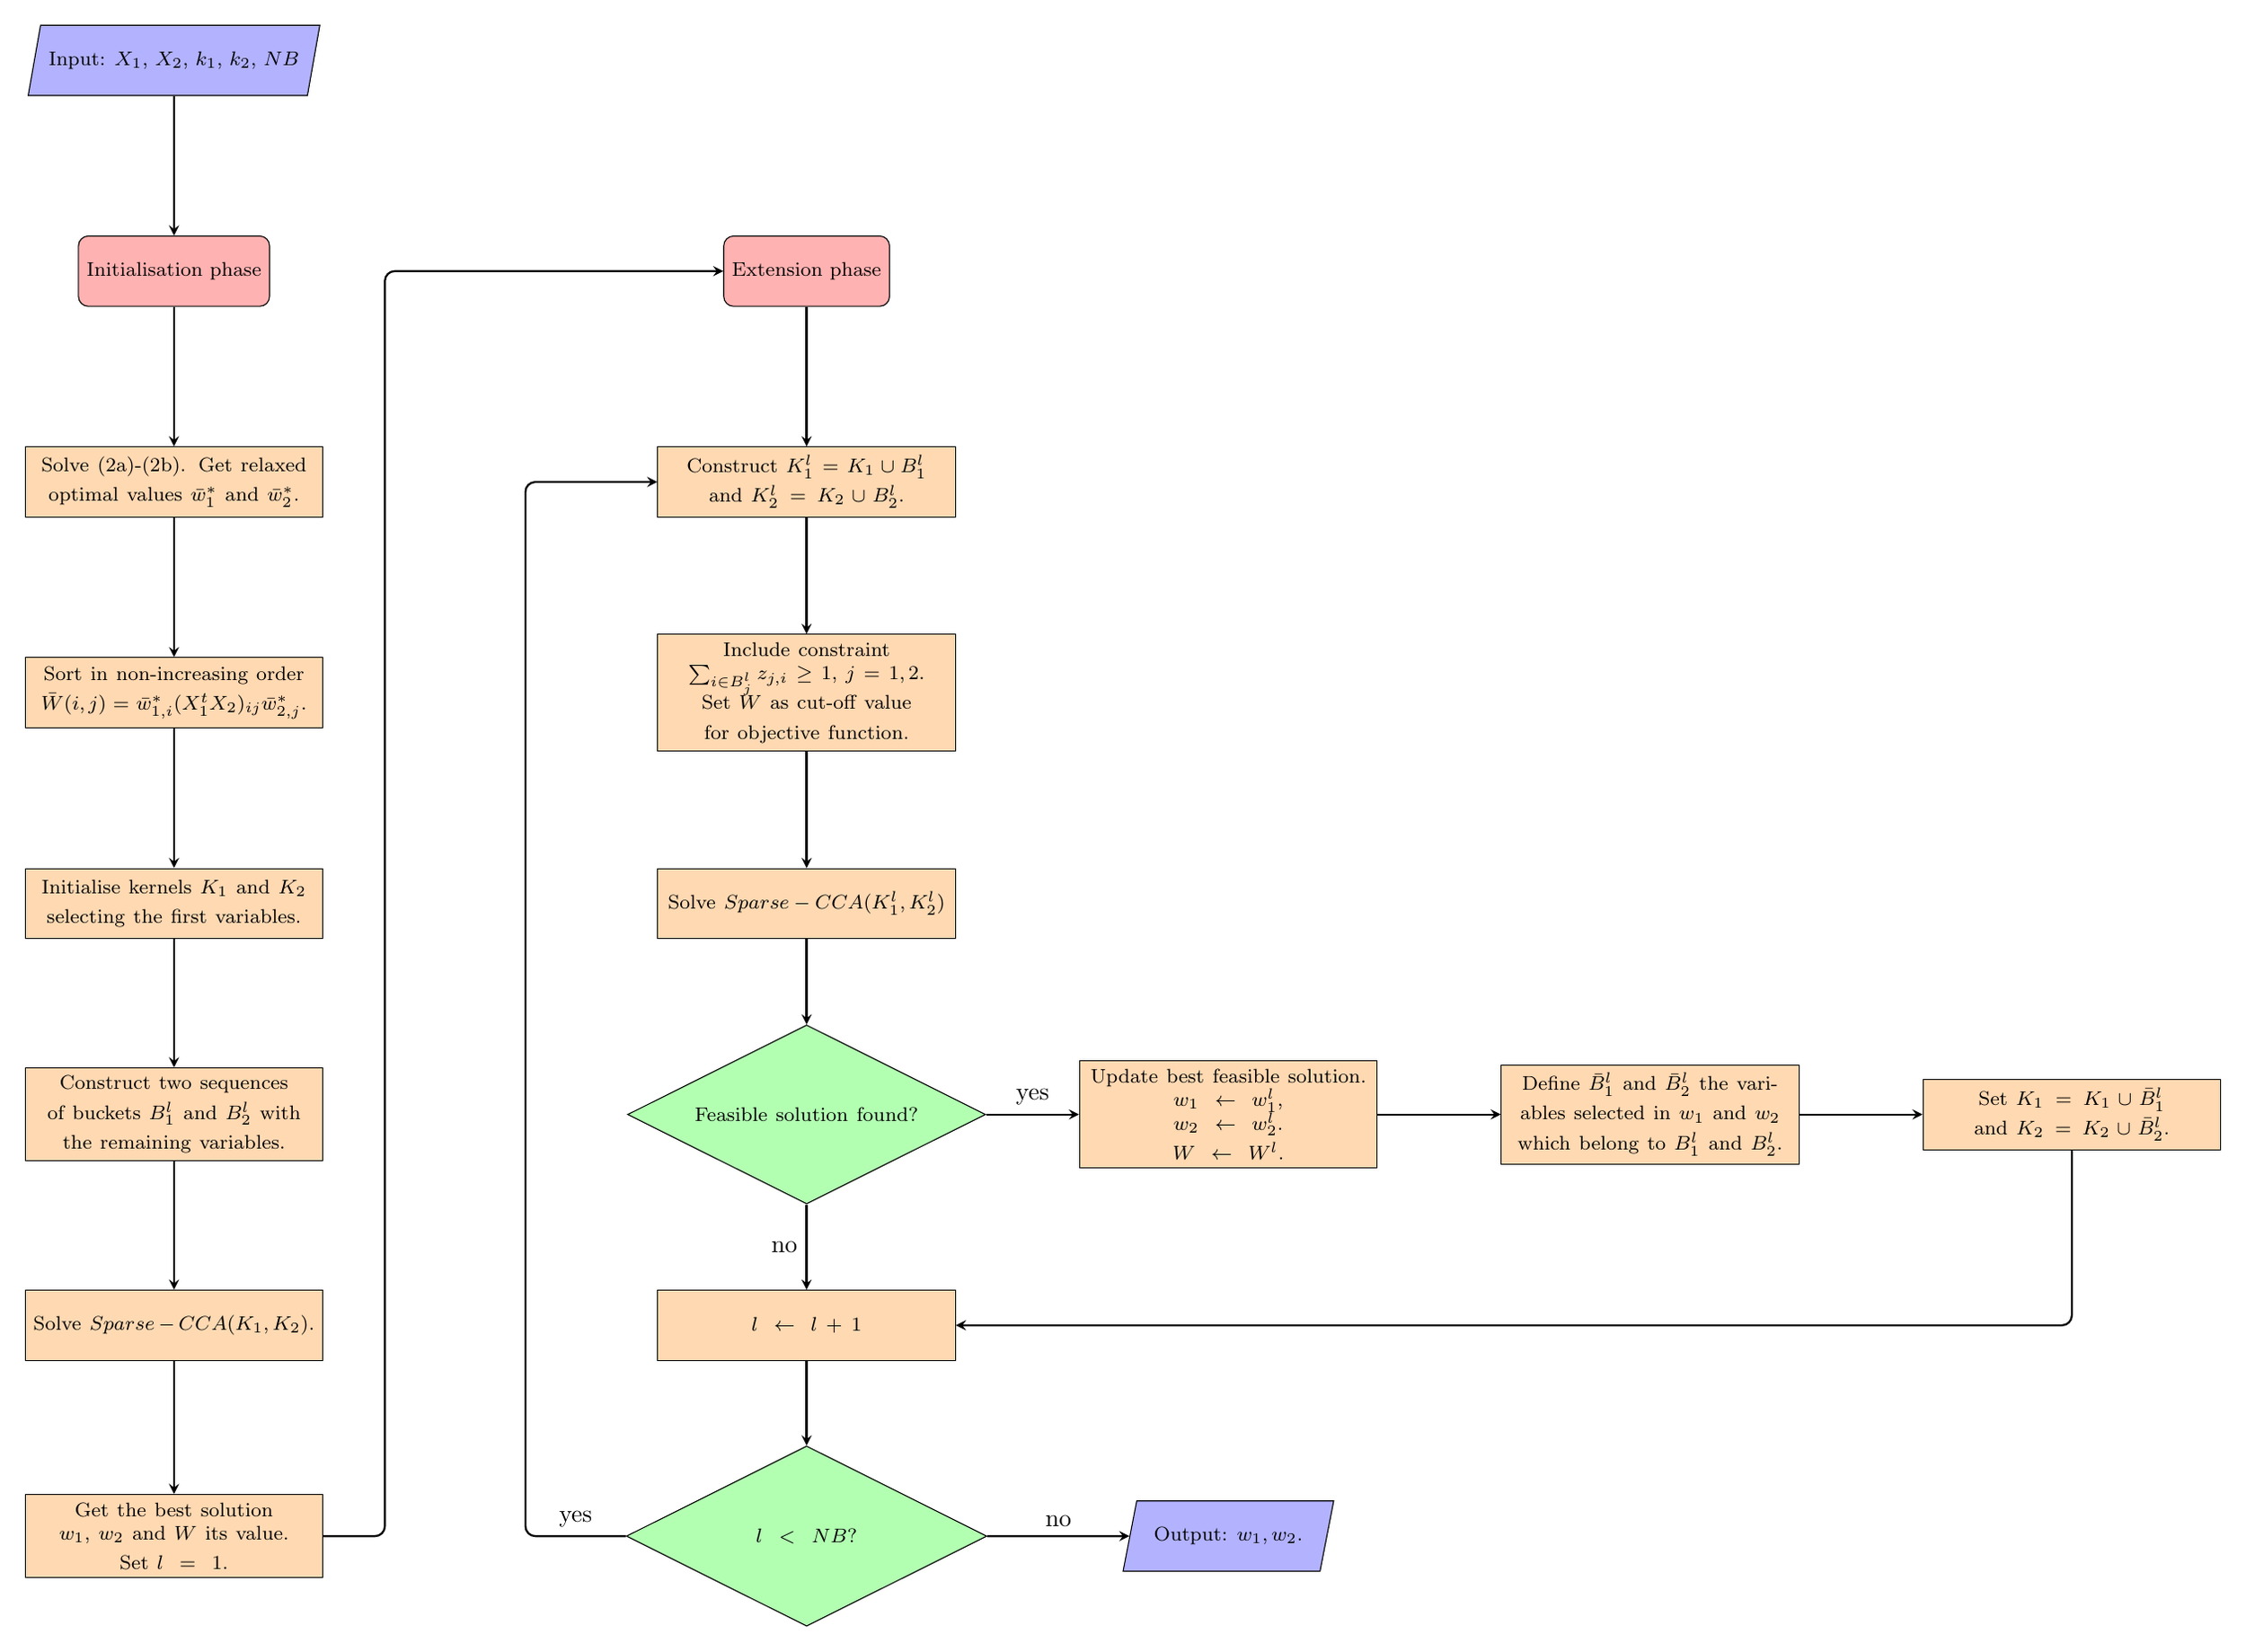
\begin{tikzpicture}[node distance=3cm, scale=1]
			
			%	\node (start) [startstop] {\footnotesize Start};
			\node (in1) [io] {\footnotesize Input: $X_1$, $X_2$, $k_1$, $k_2$, $NB$};
			
			\node (start) [startstop, below of=in1] {\footnotesize Initialisation phase};
			
			\node (pro1) [process, below of=start] {\footnotesize Solve (2a)-(2b). Get relaxed optimal values $\bar{w}_{1}^{*}$ and $\bar{w}_{2}^{*}$. };
			
			\node (pro2) [process, below of=pro1] {\footnotesize Sort in non-increasing order $\bar{W}(i, j)=\bar{w}_{1, i}^*(X_1^tX_2)_{ij}\bar{w}_{2, j}^*$.};
			
			\node (pro3) [process, below of=pro2] {\footnotesize Initialise kernels $K_1$ and $K_2$ selecting the first variables.};
			
			\node (pro4) [process, below of=pro3] {\footnotesize Construct two sequences of buckets $B_1^l$ and $B_2^l$ with the remaining variables.};
			
			\node (pro5) [process, below of=pro4] {\footnotesize Solve $Sparse-CCA(K_1, K_2)$.};
			
			\node (pro6) [process, below of=pro5] {\footnotesize Get the best solution $w_1$, $w_2$ and $W$ its value. \\Set $l=1$.};
			
			\node (start2) [startstop, right of=start, xshift=6cm] {\footnotesize Extension phase};
			\node (pro7) [process, right of=pro1, xshift=6cm] {\footnotesize Construct $K_1^l=K_1\cup B_1^l$ and $K_2^l=K_2\cup B_2^l$.};
			
			\node (pro8) [process, below of=pro7] {\footnotesize Include constraint $\sum_{i\in B_j^l} z_{j, i} \geq 1$, $j=1,2$.\\ Set $W$ as cut-off value for objective function.};
			
			\node (pro9) [process, below of=pro8] {\footnotesize Solve $Sparse-CCA(K_1^l, K_2^l)$ };
			\node (dec9) [decision, below of=pro9] {\footnotesize Feasible solution found?};
			
			\node (pro9a) [process, right of=dec9, xshift=3cm] {\footnotesize Update best feasible solution. \\ $w_1 \gets w_1^l$, \\$w_2 \gets w_2^l$.\\ $W\gets W^l$.};
			
			\node (pro9b) [process, right of=pro9a, xshift=3cm] {\footnotesize Define $\bar{B}^l_1$ and $\bar{B}^l_2$ the variables selected in $w_1$ and $w_2$ which belong to $B_1^l$ and $B_2^l$.};
			
			\node (pro9c) [process, right of=pro9b, xshift=3cm] {\footnotesize Set $K_1 = K_1\cup \bar{B}^l_1$ and $K_2=K_2\cup\bar{B}^l_2$.};
			
			\node (pro10) [process, below of=dec9] {\footnotesize $l\gets l+1$};
			\node (dec10) [decision, below of=pro10] {\footnotesize $l < NB$?};
			
			\node (out) [io, right of=dec10, xshift=3cm] {\footnotesize Output: $w_1, w_2$.};
			
			\draw [arrow] (in1) -- (start);
			\draw [arrow] (start) -- (pro1);
			\draw [arrow] (pro1) -- (pro2);
			\draw [arrow] (pro2) -- (pro3);
			\draw [arrow] (pro3) -- (pro4);
			\draw [arrow] (pro4) -- (pro5);
			\draw [arrow] (pro5) -- (pro6);
			\draw [arrow] (pro6) -- +(3,0) |- (start2);
			\draw [arrow] (start2) -- (pro7);
			\draw [arrow] (pro7) -- (pro8);
			\draw [arrow] (pro8) -- (pro9);
			\draw [arrow] (pro9) -- (dec9);
			\draw [arrow] (dec9) -- node[anchor=south] {yes} (pro9a);
			\draw [arrow] (dec9) -- node[anchor=east] {no} (pro10);
			\draw [arrow] (pro9a) -- (pro9b);
			\draw [arrow] (pro9b) -- (pro9c);
			\draw [arrow] (pro9c) |- (pro10);
			\draw [arrow] (pro10) -- (dec10);
			\draw [arrow] (dec10) -- node[anchor=south] {no} (out);
			\draw [arrow] (dec10) -- node[anchor=south] {yes} + (-4,0)  |-  (pro7);
			
			%		\draw [arrow] (dec7b) -- node[]
			
			%		\draw [arrow] (dec1) -- node[anchor=south] {no} (pro2b);
			%		\draw [arrow] (pro2b) -- (pro2c);
			%		\draw [arrow] (pro2c) |- (pro2);
			%		\draw [arrow] (pro2) -- (dec2a);
			%		\draw [arrow] (dec2a) -- node[anchor=south] {no} +(4,0) |- (out3b);
			%		\draw [arrow] (dec2a) -- node[anchor=east] {yes} (dec2b);
			%		\draw [arrow] (dec2b) -- node[anchor=south] {yes} +(4,0) |- (out3b);
			%		\draw [arrow] (dec2b) -- node[anchor=east] {no} (pro3);
			%		\draw [arrow] (pro3) -- (dec3a);
			%		\draw [arrow] (dec3a) -- node[anchor=south] {no} +(4,0) |- (out3b);
			%		\draw [arrow] (dec3a) -- node[anchor=east] {yes} (dec3b);
			%		\draw [arrow] (dec3b) -- node[anchor=south] {yes} +(4,0) -- (out3b);
			%		\draw [arrow] (dec3b) -- node[anchor=south] {no} + (-4,0)  |-  (pro2);
			%	\draw [arrow] (pro2a) -- (out1);
			%	\draw [arrow] (out1) -- (stop);
			
		\end{tikzpicture}
	\end{adjustbox}
\end{center}

\begin{center}
	\begin{adjustbox}{width=1\textwidth,height=1\textheight,keepaspectratio}
		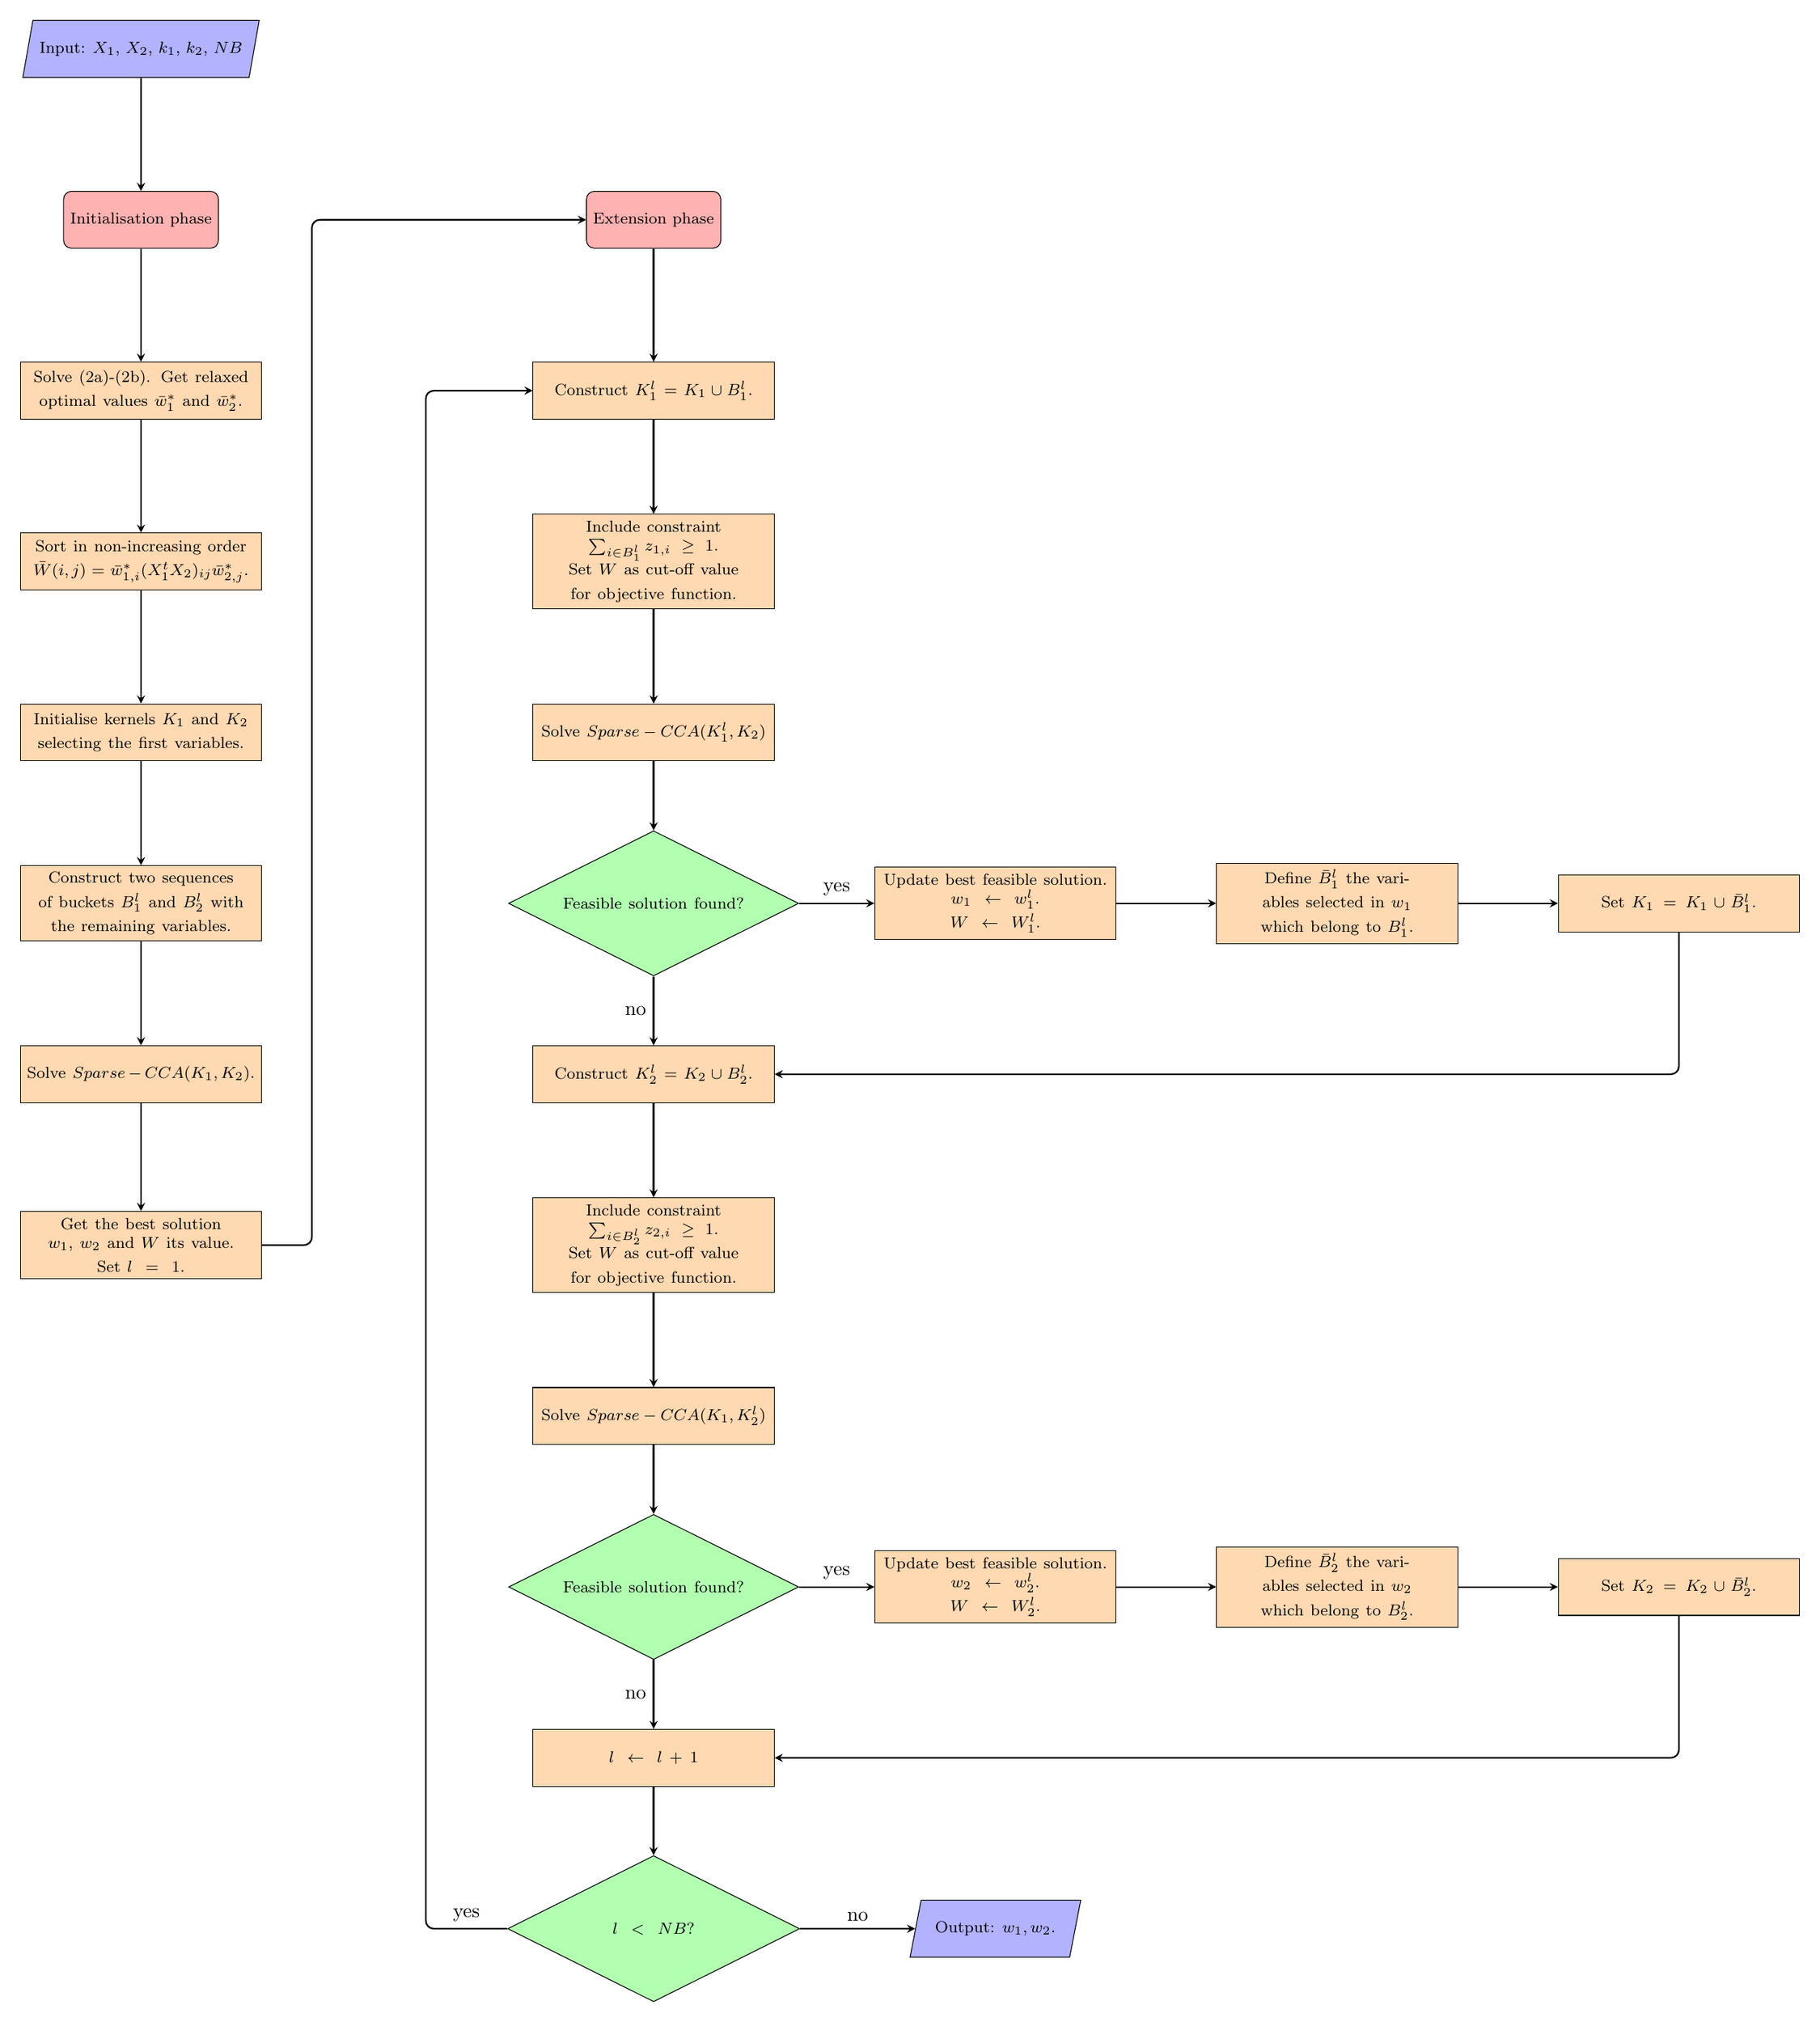
\begin{tikzpicture}[node distance=3cm, scale=1]
			
			%	\node (start) [startstop] {\footnotesize Start};
			\node (in1) [io] {\footnotesize Input: $X_1$, $X_2$, $k_1$, $k_2$, $NB$};
			
			\node (start) [startstop, below of=in1] {\footnotesize Initialisation phase};
			
			\node (pro1) [process, below of=start] {\footnotesize Solve (2a)-(2b). Get relaxed optimal values $\bar{w}_{1}^{*}$ and $\bar{w}_{2}^{*}$. };
			
			\node (pro2) [process, below of=pro1] {\footnotesize Sort in non-increasing order $\bar{W}(i, j)=\bar{w}_{1, i}^*(X_1^tX_2)_{ij}\bar{w}_{2, j}^*$.};
			
			\node (pro3) [process, below of=pro2] {\footnotesize Initialise kernels $K_1$ and $K_2$ selecting the first variables.};
			
			\node (pro4) [process, below of=pro3] {\footnotesize Construct two sequences of buckets $B_1^l$ and $B_2^l$ with the remaining variables.};
			
			\node (pro5) [process, below of=pro4] {\footnotesize Solve $Sparse-CCA(K_1, K_2)$.};
			
			\node (pro6) [process, below of=pro5] {\footnotesize Get the best solution $w_1$, $w_2$ and $W$ its value. \\Set $l=1$.};
			
			\node (start2) [startstop, right of=start, xshift=6cm] {\footnotesize Extension phase};
			\node (pro7) [process, right of=pro1, xshift=6cm] {\footnotesize Construct $K_1^l=K_1\cup B_1^l$.};
			
			\node (pro8) [process, below of=pro7] {\footnotesize Include constraint $\sum_{i\in B_1^l} z_{1, i} \geq 1$.\\ Set $W$ as cut-off value for objective function.};
			
			\node (pro9) [process, below of=pro8] {\footnotesize Solve $Sparse-CCA(K_1^l, K_2)$ };
			\node (dec9) [decision, below of=pro9] {\footnotesize Feasible solution found?};
			
			\node (pro9a) [process, right of=dec9, xshift=3cm] {\footnotesize Update best feasible solution. \\ $w_1 \gets w_1^l$. \\ $W\gets W^l_1$.};
			
			\node (pro9b) [process, right of=pro9a, xshift=3cm] {\footnotesize Define $\bar{B}^l_1$ the variables selected in $w_1$ which belong to $B_1^l$.};
			
			\node (pro9c) [process, right of=pro9b, xshift=3cm] {\footnotesize Set $K_1 = K_1\cup \bar{B}^l_1$.};
			
			\node (pro10) [process, below of=dec9] {\footnotesize Construct $K_2^l=K_2\cup B_2^l$.};
			
			\node (pro11) [process, below of=pro10] {\footnotesize Include constraint $\sum_{i\in B_2^l} z_{2, i} \geq 1$.\\ Set $W$ as cut-off value for objective function.};
			
			\node (pro12) [process, below of=pro11] {\footnotesize Solve $Sparse-CCA(K_1, K_2^l)$ };
			\node (dec12) [decision, below of=pro12] {\footnotesize Feasible solution found?};
			\node (pro12a) [process, right of=dec12, xshift=3cm] {\footnotesize Update best feasible solution. \\ $w_2 \gets w_2^l$. \\ $W\gets W^l_2$.};
			
			\node (pro12b) [process, right of=pro12a, xshift=3cm] {\footnotesize Define $\bar{B}^l_2$ the variables selected in $w_2$ which belong to $B_2^l$.};
			
			\node (pro12c) [process, right of=pro12b, xshift=3cm] {\footnotesize Set $K_2 = K_2\cup \bar{B}^l_2$.};
			
			\node (pro13) [process, below of=dec12] {\footnotesize $l\gets l+1$};
			\node (dec13) [decision, below of=pro13] {\footnotesize $l < NB$?};
			
			\node (out) [io, right of=dec13, xshift=3cm] {\footnotesize Output: $w_1, w_2$.};
			
			\draw [arrow] (in1) -- (start);
			\draw [arrow] (start) -- (pro1);
			\draw [arrow] (pro1) -- (pro2);
			\draw [arrow] (pro2) -- (pro3);
			\draw [arrow] (pro3) -- (pro4);
			\draw [arrow] (pro4) -- (pro5);
			\draw [arrow] (pro5) -- (pro6);
			\draw [arrow] (pro6) -- +(3,0) |- (start2);
			\draw [arrow] (start2) -- (pro7);
			\draw [arrow] (pro7) -- (pro8);
			\draw [arrow] (pro8) -- (pro9);
			\draw [arrow] (pro9) -- (dec9);
			\draw [arrow] (dec9) -- node[anchor=south] {yes} (pro9a);
			\draw [arrow] (dec9) -- node[anchor=east] {no} (pro10);
			\draw [arrow] (pro9a) -- (pro9b);
			\draw [arrow] (pro9b) -- (pro9c);
			\draw [arrow] (pro9c) |- (pro10);
			\draw [arrow] (pro10) -- (pro11);
			\draw [arrow] (pro11) -- (pro12);
			\draw [arrow] (pro12) -- (dec12);
			\draw [arrow] (dec12) -- node[anchor=south] {yes} (pro12a);
			\draw [arrow] (dec12) -- node[anchor=east] {no} (pro13);
			\draw [arrow] (pro12a) -- (pro12b);
			\draw [arrow] (pro12b) -- (pro12c);
			\draw [arrow] (pro12c) |- (pro13);
			\draw [arrow] (pro13) -- (dec13);
			\draw [arrow] (dec13) -- node[anchor=south] {no} (out);
			\draw [arrow] (dec13) -- node[anchor=south] {yes} + (-4,0)  |-  (pro7);
			
			%		\draw [arrow] (dec7b) -- node[]
			
			%		\draw [arrow] (dec1) -- node[anchor=south] {no} (pro2b);
			%		\draw [arrow] (pro2b) -- (pro2c);
			%		\draw [arrow] (pro2c) |- (pro2);
			%		\draw [arrow] (pro2) -- (dec2a);
			%		\draw [arrow] (dec2a) -- node[anchor=south] {no} +(4,0) |- (out3b);
			%		\draw [arrow] (dec2a) -- node[anchor=east] {yes} (dec2b);
			%		\draw [arrow] (dec2b) -- node[anchor=south] {yes} +(4,0) |- (out3b);
			%		\draw [arrow] (dec2b) -- node[anchor=east] {no} (pro3);
			%		\draw [arrow] (pro3) -- (dec3a);
			%		\draw [arrow] (dec3a) -- node[anchor=south] {no} +(4,0) |- (out3b);
			%		\draw [arrow] (dec3a) -- node[anchor=east] {yes} (dec3b);
			%		\draw [arrow] (dec3b) -- node[anchor=south] {yes} +(4,0) -- (out3b);
			%		\draw [arrow] (dec3b) -- node[anchor=south] {no} + (-4,0)  |-  (pro2);
			%	\draw [arrow] (pro2a) -- (out1);
			%	\draw [arrow] (out1) -- (stop);
			
		\end{tikzpicture}
	\end{adjustbox}
\end{center}

\end{document}